\documentclass[conference]{IEEEtran}
\usepackage[english]{babel}
\usepackage[utf8]{inputenc}
\usepackage[T1]{fontenc}
\usepackage{mathtools}
\usepackage{amssymb}
\usepackage{graphicx}

\newcommand{\equref}[1]{Equation~\ref{#1}}
\newcommand{\figref}[1]{Figure~\ref{#1}}
\newcommand{\apref}[1]{Appendix~\ref{#1}}
\newcommand{\secref}[1]{Section~\ref{#1}}
\newcommand{\dindex}[3]{#1_{#2,\;#3}}

\newcommand{\url}[1]{Web address goes here}

\newcommand{\innerimage}[3]{
  \includegraphics[clip=true, trim=#2, width=\linewidth]{assets/#1.pdf}
  \caption{#3}
  \label{fig:#1}
}

\newcommand{\image}[3]{
  \begin{figure}
    \centering
    \innerimage{#1}{#2}{#3}
  \end{figure}
}


\newcommand{\ssdtc}{Steady-State Dynamic Temperature Curve}

\title{Steady-State Dynamic Temperature Analysis for Multiprocessor Systems}
\author{Min Bao, Petru Eles, Zebo Peng, and Ivan Ukhov}

\begin{document}
  \maketitle

  \begin{abstract}
      An accurate and fast temperature estimation of a multiprocessor system is not an easy goal to achieve. This is mainly due to the fact that the underlying process has a significantly complex nature. The temperature variation within a die depends on a lot of different parameters, both extrinsic (e.g., the ambient conditions) and intrinsic (e.g., the dynamic power consumption and power leakage). The problem becomes even more severe when one takes a little step further and puts it inside of an optimization loop where this type of estimation has to be performed thousands of times. In this case, the solution should be not only accurate, but also computationally cheap to find. In this paper we propose such a technique that satisfies both criteria, accuracy and speed.
  Our particular focus of interest is \emph{multiprocessor} system-on-chips that have \emph{periodic} power and, consequently, temperature profiles (for instance, embedded systems executing periodic applications). The proposed solution is \emph{analytical}, therefore, it is \emph{exact} from the perspective of the underlying model, also it is \emph{fast} enough to be used in a wide range of search heuristics. In order to demonstrate our approach to the steady-state dynamic temperature analysis, we perform the temperature-aware reliability optimization of multiprocessor systems with periodic applications.
  The thermal model that we use in our analysis is \emph{leakage-aware}, since the power leakage is still an important issue that should be carefully taken into account. The reliability model, that we have chosen as an example, is based on the thermal cycling failure mechanism.
  The optimization process is held by a genetic algorithm that varies task allocation and scheduling in order to achieve the longest mean time to failure of the system within curtain constrains. We also conduct a multi-objective optimization with the energy consumption as one additional goal. In this case, the solution is a Pareto front for the designer to choose from.

  \end{abstract}

  \section{Introduction}
  \subsection{Temperature Variation}
Morden policies for prevening temperature runaways and decreasing energy consumption, within such tecniques as dynamic power management (DPM) and dynamic voltage and frequency scaling (DVFS), keep puzzling embedded system architects with a constantly increasing strength. These and similar approaches may cause considerable temperature fluctuations within a multiprocessor system-on-chip (MPSoC), therefore, dramatically decreasing its reliability \cite{mihic2004}, \cite{simunic2005}.

The importance of the temperature distribution over ICs has been widely studied in the literature \cite{lu2004}. Hence, a large number of different methods for performance and energy optimization imposes the maximal temperature constrain. In this essence, the need of fast and accurate methods for obtaining temperature profiles becomes urgent.

In this paper we consider the HotSpot thermal model \cite{huang2006} and propose an extremely fast way to calculate the steady-state dynamic temperature curve (SSDTC) of an embedded system that executes a set of periodic tasks.

In order to demonstrate our approach, we perform the energy optimization with a constrain on the spatial temperature gradient within a die. The constrain is satisfied with the help of SSDTC that delivers the diapason of the temperature fluctuation. The optimization problem is solved through the mapping and scheduling based on genetic algorithms and the list scheduler described in \cite{schmitz2004}.

\subsection{Motivational Example}
TODO.


  \section{Preliminaries} \label{sec:preliminaries}
  The proposed SSDTA technique is based on the well-known RC thermal model that employs the analogy between electrical and thermal circuits. According to this model, the temperature behaviour can be predicted by constracting equivalent RC thermal circuits where electrical current, voltage, resistance, and capacitance are replaced by heat flow, temperature, thermal resistance, and thermal capacitance, correspondingly. The heat equation in this model takes the following matrix form:
\begin{equation} \label{eq:thermal-ode}
  C \frac{dT}{dt} + G T = P
\end{equation}
where $T$ is a vector of temperature, $C$ is the thermal capacitance matrix, $G$ is the thermal conductance matrix (equal to $R^{-1}$, where $R$ is the resistance matrix), and $P$ is a vector of the power dissipation (the source of heat). $C$ and $G$ are $N_n \times N_n$ matrices, $T$ and $P$ are vectors of the length $N_n$, where $N_n$ is the number of thermal nodes. For convenience, in the rest of the paper we use the following denotation:
\begin{equation} \label{eq:initial}
  C \frac{dT}{dt} = A T + B
\end{equation}

An equivalent circuit of a multiprocessor system with a thermal package can be built in a wide range of different ways. Therefore, the number of thermal nodes $N_n$, as well as the conductance and capacitance matrices, depends on a particular realization of the model, i.e., its granularity. For instance, the wide spread thermal simulator HotSpot \cite{huang2006} includes two different implementations, so-called block and grid models. In the block model each core of a multiprocessor system is given one thermal node, while with the grid model the whole die is covered is an adjustable mesh of thermal nodes. Both models have a number of extra nodes for the thermal package of the die which includes the thermal interface material, heat spreader, and heat sink. For example, in case of the block model with $N_p$ processing elements, the total number of thermal nodes can be computed according to the following equation \cite{rao2008}:
\begin{equation} \label{eq:nodes}
  N_n = 4 \times N_p + 12
\end{equation}

The choice of a particular model depends on a desired accuracy. Without loss of generality, we shall use the block model of HotSpot in our experiments.


  \section{Prior Work and Motivation} \label{sec:motivation}
  Consider an application with six tasks, denoted ``T0''--``T5'', and a heterogeneous architecture with two cores, labeled ``PE0'' and ``PE1''. The task graph of the application is given in \figref{fig:task-graph} along with the execution times for both cores. The period of the application is 0.06 seconds. A first alternative mapping and schedule, and the resulting SSDTP are shown at the top of \figref{fig:motivation} (where the hight of a task represents its relative dynamic power consumption). It can be observed that initially PE0 is experiencing three thermal cycles. If we change the mapping of T5 and move it to PE1, we achieve two thermal cycles of PE0 instead of three. Finally, if we vary the schedule as well and change the order of T1 and T3, the number of cycles of PE0 becomes one. Using the reliability model from \secref{sec:reliability-model}, we observe improvements in the MTTF of 44.69\% and 54.53\%, respectively, relative to the initial configuration.
\begin{figure}
  \centering
  \subfloat[The task graph.]{
    \label{fig:task-graph}
    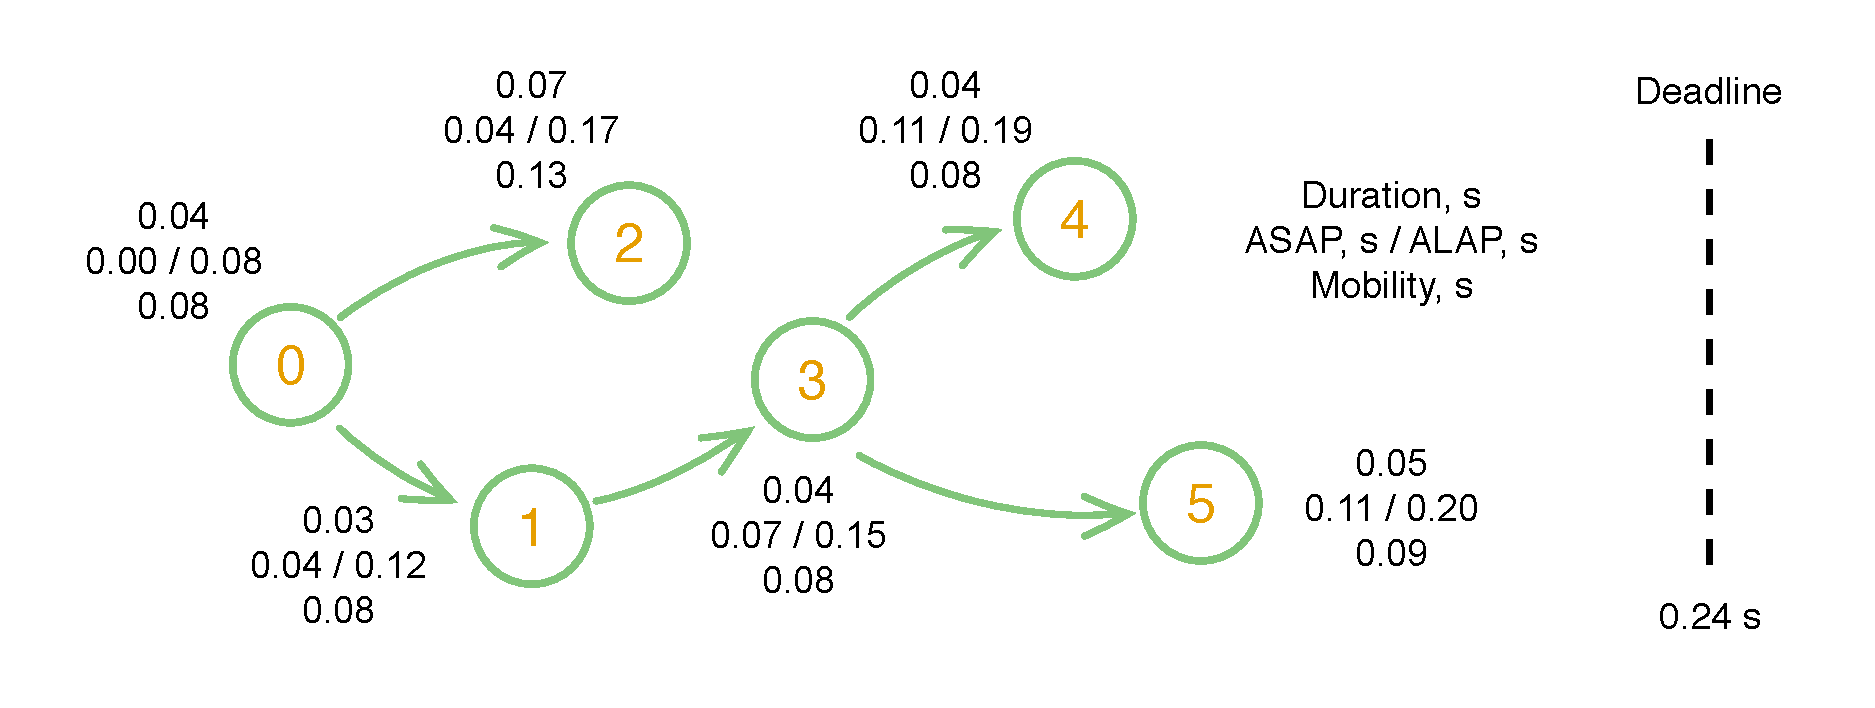
\includegraphics[width=0.8\linewidth]{assets/task-graph.pdf}
  }
  \vspace{-15pt}

  \subfloat[Alternative mappings and schedules.]{
    \label{fig:motivation}
    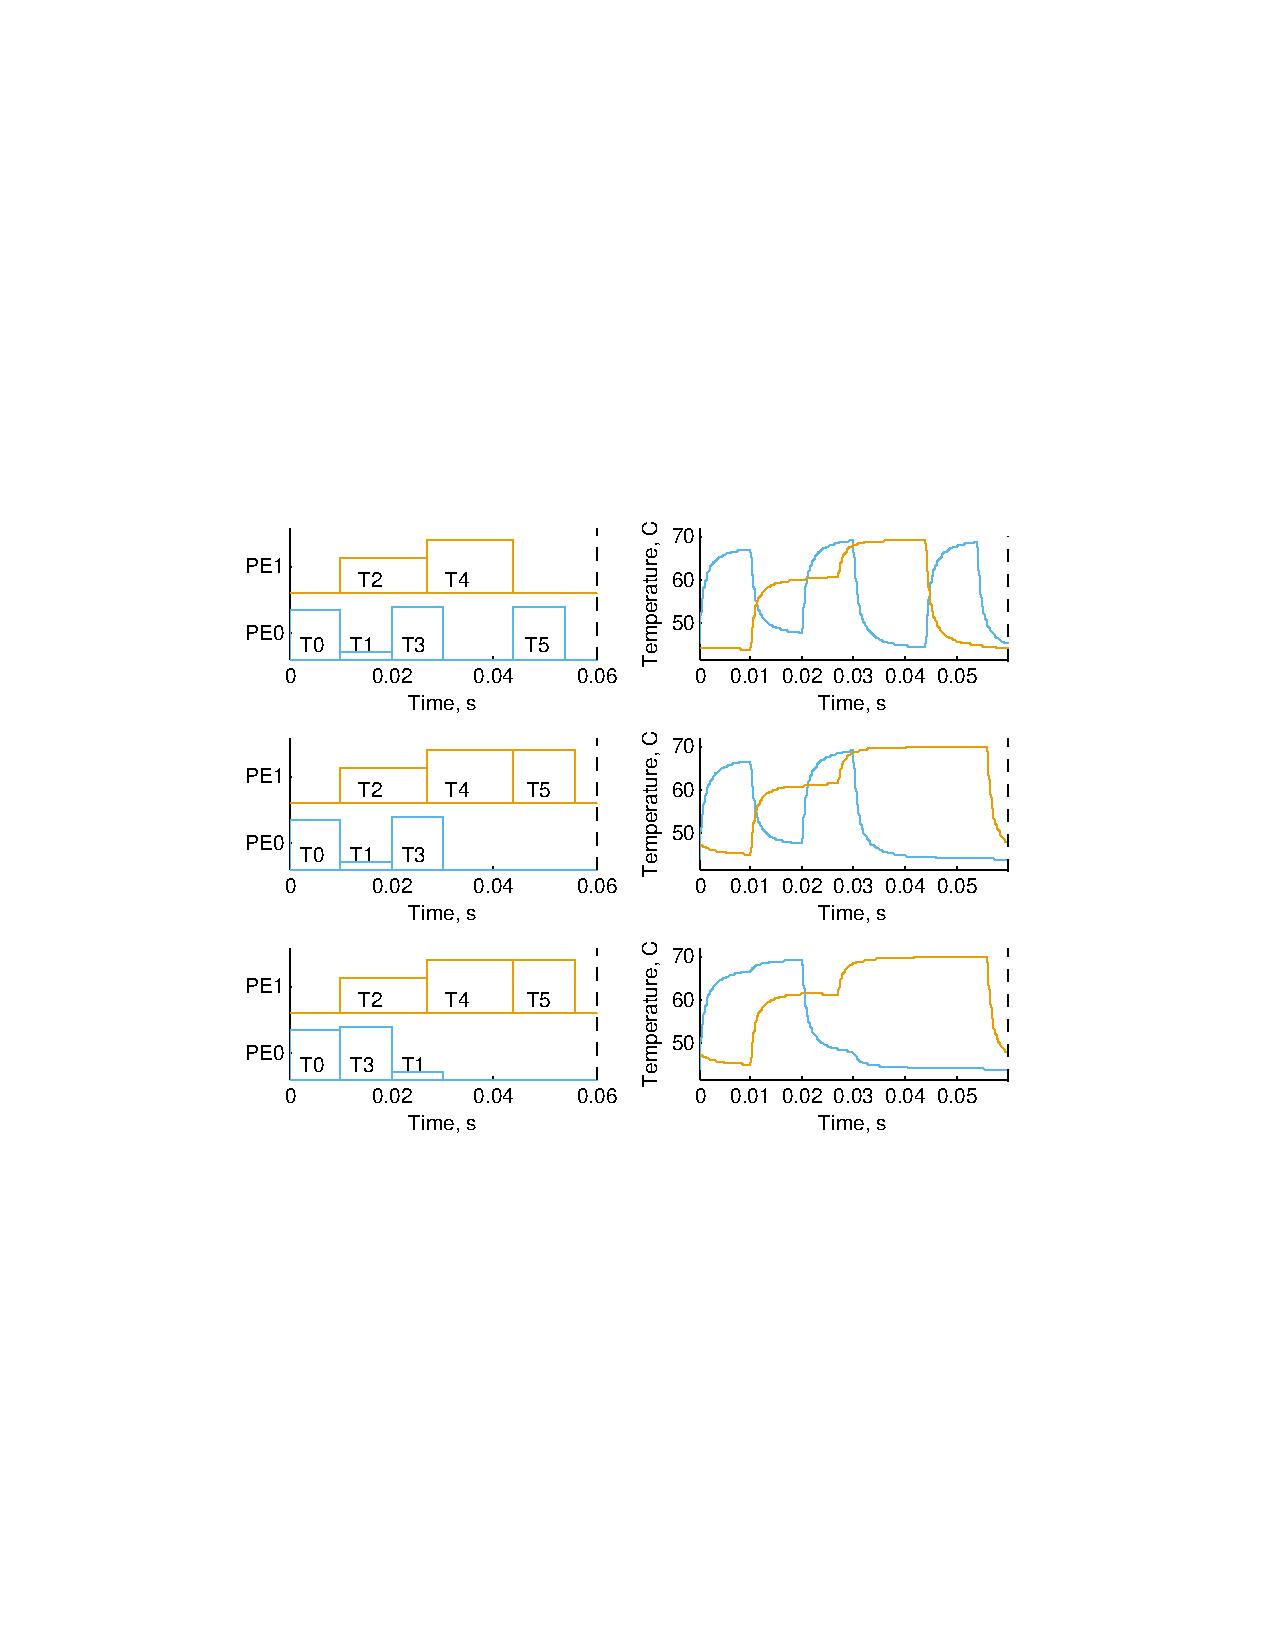
\includegraphics[width=0.8\linewidth]{assets/motivation.pdf}
  }
  \vspace{5pt}
  \caption{Motivational example.}
  \vspace{15pt}
\end{figure}


  \section{Problem Formulation} \label{sec:problem}
  Consider a multicore system that consists of $N_p$ processing elements $\Pi = \{ \pi_k: k = 0 \dots N_p - 1 \}$ and executes a periodic application with a period $\mathcal{T}$. An equivalent RC thermal circuit of the system is constructed and contains $N_n$ thermal nodes. The application period is discretized into $N_s$ intervals \mbox{$\Delta \mathcal{T} = \{ \Delta t_i: \: i = 0 \dots N_s - 1 \}$} in such a way that the dynamic power dissipation and temperature of each node are assumed to be constant within an interval. The discrete dynamic power profile is defined as \mbox{$\mathbb{P}_{dyn} = \{ P_{ij}: \: i = 0 \dots N_s - 1, \: j = 0 \dots N_n - 1 \}$} where $P_{ij}$ is the dynamic power dissipation during the $i$th time interval of the $j$th thermal node. The profile is denoted as $\mathbb{P}_{\: dyn}^{\:act}$ when only active nodes are included. After the stabilization process is finished and the steady state is reached, the corresponding temperature profile becomes periodic and is defined as \mbox{$\mathbb{T} = \{ T_{ij}: \: i = 0 \dots N_s - 1, \: j = 0 \dots N_n - 1 \}$} where $T_{ij}$ is the temperature in the $i$th time interval of the $j$th node. The profile is called the Steady-State Dynamic Temperature Profile (SSDTP).

Given:
\begin{itemize}
  \item A multicore system with a set of processing elements $\Pi$ executing a periodic application.
  \item The dynamic power profile $\mathbb{P}_{\:dyn}^{\:act}$ of the system with discretization $\Delta \mathcal{T}$.
  \item The floorplan of the chip, i.e., the location and size of the processing elements $\Pi$.
  \item The configuration of the thermal package, i.e., dimensions of the thermal interface material, heat spreader, and heat sink.
  \item The thermal parameters of the die and package, e.g., the thermal conductivity and thermal capacitance.
\end{itemize}

Find:
\begin{itemize}
  \item The corresponding periodic temperature profile $\mathbb{T}$ of the system when the steady state is reached.
\end{itemize}

Reasonable requirements for a solution are speed and accuracy, since the temperature analysis is often a part of an intensive optimization procedure where the SSDTP is to be computed thousands of times. Such a problem is described in \secref{sec:reliability}.


  \section{Solutions with the HotSpot Simulator} \label{sec:hotspot-solution}
  Before going to the proposed solution, we first discuss the available state of the art techniques.

\subsection{Iterative Simulation} \label{sec:hotspot-iterative-solution}
A rough approximation of the SSDTP can be obtained by running a temperature simulator over successive periods of the application until it can be assumed that the system has reached the thermal steady state. The simulator performs the transient temperature analysis where the common approach is to solve \equref{eq:fourier-model} numerically, e.g., using the fourth-order Runge-Kutta method \cite{press2007}.

\iimage{hotspot-error}{40 230 40 230}{Normalized RMSE over successive iterations with HotSpot.}
\begin{itable}{parameters}{|l|r|}
  {Parameters of the Die and Thermal Package}
  {The thermal parameters (i.e., thermal conductivity, specific heat, convection resistance and capacitance) used in our experiments are equal to the default ones found in HotSpot 5.0 \cite{huang2008}.}
  \hline
  Parameter & Value \\
  \hline
  \hline
  Ambient temperature                   &   27 ${}^\circ C$ \\
  Convection capacitance                & 140.4 J/K \\
	Convection resistance                 & 0.1 K/W \\
  Die thickness                         & 0.15 $mm$ \\
  Thermal interface material thickness  & 0.02 $mm$ \\
  Heat spreader side                    &   20 $mm$ \\
  Heat spreader thickness               &    1 $mm$ \\
  Heat sink side                        &   30 $mm$ \\
  Heat sink thickness                   &   15 $mm$ \\
  \hline
\end{itable}
The number of simulations required to reach the SSDTP depends on the thermal characteristics of the system. In order to illustrate this aspect, we have considered an application with the period of 0.5 seconds running on five hypothetical platforms with core areas between 1 and 25 $mm^2$. The configuration of the die itself and thermal package is given in \tabref{tab:parameters}. We have run the temperature simulation with HotSpot \cite{huang2008} for 50 successive periods of the application. The temperature profile in each period has been compared with the real SSDTP obtained with our analytical approach (\secref{sec:analytical-solution}) and the normalized Root Mean Square Error (RMSE) has been calculated. The result is shown in \figref{fig:hotspot-error}. It can be observed that the number of successive periods over which the temperature simulation has to be performed in order to achieve a satisfactory level of accuracy is significant for the majority of configurations. For a 9 $mm^2$ die, for example, after 15 iterations, the normalized RMSE is still close to 20\%. This leads to large computation times, making it difficult to apply the technique inside an intensive optimization loop.

\subsection{Steady-State Approximation (SSA)} \label{sec:steady-state-approximation}
\iimage{steady-state-approximation}{-30 10 -30 10}{A SSDTP and its approximation with the SSA.}
An approximation method of the SSDTP has been proposed in \cite{huang2009}. Instead of solving the system of differential equations given by \equref{eq:fourier-model}, it is assumed that during each time interval $\Delta t_i$ in which the power is constant the whole system stays in its steady state. In this case the derivative \mbox{$d\v{T}/dt = 0$} and the temperature can be calculated as $\v{T}_i = \m{G}^{-1} \v{P}_i$.

The result is a stepwise temperature curve where each step corresponds to the steady-state temperature $\v{T}_i$ that would be reached if the constant power $\v{P}_i$ was applied for a sufficiently long time. An example of such an approximation (SSA) along with the corresponding SSDTP for an application with 10 tasks and period of 0.1 seconds is given in \figref{fig:steady-state-approximation}. The die area is 25 $mm^2$, the configuration of the chip is the same as in \tabref{tab:parameters}. The reduced accuracy of the approximation is due to the mismatch between the actual temperature within each interval $\Delta t_i$ and the hypothetical steady-state temperature. The inaccuracy depends on the thermal characteristics of the respective platform and on the application itself. To illustrate this, we have generated five applications with periods between 0.01 and 1 seconds and computed approximated SSDTPs for die areas between 1 and 25 $mm^2$. The normalized RMSE relative to the correct SSDTP is shown in \figref{fig:steady-state-error}. It can be seen that, e.g., for a die area of 10 $mm^2$ and a period of 100 $ms$ the normalized RMSE \todo{with the} SSA is close to 40\%.
\iimage{steady-state-error}{40 230 40 230}{Normalized RMSE as a function of die area with the SSA.}


  \section{Proposed Analytical Solution} \label{sec:analytical-solution}
  \subsection{Analytical Solution}
In order to resolve the problem, we use an analytical approach. The direct solution of \equref{eq:initial} is given by the following equation:
\begin{equation} \label{eq:solution}
  T(t) = e^{C^{-1}A t} \; T_0 + (C^{-1} A)^{-1}(e^{C^{-1}A t} - I)C^{-1} B
\end{equation}

The solution provides us with the transient temperature and holds only when the power vector $B$ is constant. If it is not the case, we need to simulate shorter time intervals where this assumption can take place. Before going to the steady-state case, we perform one important adjustment to the system in order to be more efficient in our future calculations. According to \equref{eq:solution}, we need to compute the matrix exponential of the matrix $C^{-1} A t$. It would be much easier to accomplish if the matrix were symmetric, because a real symmetric matrix is \emph{diagonalizable} and has \emph{independent} (orthogonal) real eigenvectors:
\begin{equation} \label{eq:eigenvalue-decomposition}
  M = U \Lambda U^T
\end{equation}
where $M$ is a real symmetric matrix, $U$ is a square matrix of the eigenvectors of $M$, $\Lambda$ is a diagonal matrix composed of the eigenvalues of $M$ ($\lambda_i$), the equation itself is called the eigenvalue decomposition. Once we have such decomposition, the matrix exponential becomes a trivial task:
\begin{align}
  & e^M = e^{U \Lambda U^T} = U \: e^{\Lambda} \: U^T \nonumber \\
  & e^{\Lambda} = \left[
      \begin{array}{ccc}
        e^{\lambda_0} & \cdots & 0 \\
        \vdots & \ddots & \vdots \\
        0 & \cdots & e^{\lambda_{n - 1}}
      \end{array}
    \right] \nonumber
\end{align}

Hence, instead of $C^{-1} A$ in front of the variable vector we want to have a symmetry matrix. In order to achieve this, we perform the following substitution:
\begin{align*}
  Y & = C^{\frac{1}{2}} T \\
  D & = C^{-\frac{1}{2}} A \: C^{-\frac{1}{2}} \\
  E & = C^{-\frac{1}{2}} B
\end{align*}
with the result:
\begin{align}
  \frac{dY}{dt} & = D \: Y + E \nonumber \\
  Y(t) & = e^{D t} Y_0 + D^{-1} (e^{D t} - I) E \label{eq:modified-solution} \\
  T(t) & = C^{-\frac{1}{2}} Y(t) \label{eq:finalization}
\end{align}

In this case, $D$ is a symmetric matrix, therefore, it will be easier to find the matrix exponential of $D \: t$ using the above-mentioned eigenvalue decomposition (\equref{eq:eigenvalue-decomposition}):
\[
  e^{D t} = U \: e^{\Lambda t} \: U^T = U \left[
      \begin{array}{ccc}
        e^{t \lambda_0} & \cdots & 0 \\
        \vdots & \ddots & \vdots \\
        0 & \cdots & e^{t \lambda_{N_n - 1}}
      \end{array}
    \right] U^T
\]

Now we shift our focus at the power profile $B$ and come closer to the SSDTP. Each row of $B$ corresponds to a particular time interval $\triangle t_i$ and represents the power consumption $B_i$ during this interval of all processing elements. Each step $i = 0 \dots N_s - 1$ of the iterative process we have a pair $(\triangle t_i, B_i)$ which gives us a temperature vector $T_i$ according to \equref{eq:modified-solution} where $t = \triangle t_i$. The iterative process can be described as the following:
\begin{align}
  & Y_{i+1} = K_i \: Y_i + G_i \: B_i \label{eq:recurrent-equation} \\
  & K_i = e^{D \: \triangle t_i} \nonumber \\
  & G_i = D^{-1} \left( e^{D \triangle t_i} - I \right) C^{-\frac{1}{2}} \nonumber
\end{align}

Since we perform the eigenvalue decomposition of D (\equref{eq:eigenvalue-decomposition}), $D^{-1}$ can be efficiently computed in the following way:
\[
  D^{-1} = U \: \Lambda^{-1} \: U^T = U \left[
      \begin{array}{ccc}
        \frac{1}{\lambda_0} & \cdots & 0 \\
        \vdots & \ddots & \vdots \\
        0 & \cdots & \frac{1}{\lambda_{N_n - 1}}
      \end{array}
    \right] U^T \\
\]
therefore:
\begin{align*}
  G_i & = U \: \Lambda^{-1} \: U^T \left(U \: e^{\Lambda \triangle t_i} \: U^T - U \: U^T \right) C^{-\frac{1}{2}} = \\
      & = U \left[
        \begin{array}{ccc}
          \frac{e^{\triangle t_i \: \lambda_0} - 1}{\lambda_0} & \cdots & 0 \\
          \vdots & \ddots & \vdots \\
          0 & \cdots & \frac{e^{\triangle t_i \: \lambda_{N_n - 1}} - 1}{\lambda_{N_n - 1}}
        \end{array}
      \right] U^T \: C^{-\frac{1}{2}}
\end{align*}

Consequently, in order to find SSDTC, we need to solve the following system of linear equations:
\[
  \begin{cases}
    K_0 \: Y_0 - Y_1 & = -Q_0 \\
    ... \\
    K_{N_s - 1} \: Y_{N_s - 1} - Y_{N_s} & = -Q_{N_s - 1}
  \end{cases}
\]
where $Q_i = G_i \: B_i$. Also we should take into account the boundary condition which ensures that the temperature has the same values on both sides of the curve:
\begin{equation} \label{eq:boundary-condition}
  Y_0 = Y_{N_s}
\end{equation}

Hence, the system of linear equations takes the following form:
\[
  \begin{cases}
    K_0 \: Y_0 - Y_1 & = -Q_0 \\
    ... \\
    -Y_0 + K_{N_s - 1} \: Y_{N_s - 1} & = -Q_{N_s - 1}
  \end{cases}
\]

To get the whole picture, the system can be written as:
\begin{align}
  & \mathbb{A} \: \mathbb{Y} = \mathbb{B} \label{eq:system} \\
  & \mathbb{A} = \left[
    \begin{array}{ccccc}
      K_0 & -I & 0 & \cdots & 0 \\
      0 & K_1 & -I &  & \vdots \\
      \vdots &  & \ddots & -I & 0 \\
      0 &  &  & K_{N_s - 2} & -I \\
      -I & 0 & \cdots & 0 & K_{N_s - 1}
    \end{array}
  \right] \nonumber \\
  & \mathbb{Y} = \left[
    \begin{array}{c}
      Y_0 \\
      \vdots \\
      Y_{N_s - 1}
    \end{array}
  \right] \nonumber \\
  & \mathbb{B} = \left[
    \begin{array}{c}
      -Q_0 \\
      \vdots \\
      -Q_{N_s - 1}
    \end{array}
  \right] \nonumber
\end{align}

where $\mathbb{A}$ is a square matrix of the dimensions $N_n N_s \times N_n N_s$. $\mathbb{Y}$ and $\mathbb{B}$ are vectors of the length $N_n N_s$.

Apparently, we have obtained a regular system of liner equations with the SSDTP as its solution ($Y$ should also be processed with \equref{eq:finalization} in order to return back to $T$). The first straight-forward way to resolve the system is to use the LU factorization (decomposition). The problem here is that such systems could be extremely large, especially when we want to achieve a higher level of accuracy and, therefore, the power profile contains a lot of steps $N_s$. Each new step is $N_n$ new equations in the system given by \equref{eq:system}. Also the complexity grows very rapidly with the number of processing elements $N_p$, since in the HotSpot thermal model the number of thermal nodes $N_n$ dependents on it according to the equation \cite{rao2008}:
\[
  N_n = 4 N_p + 12
\]

Therefore, \emph{each} new processing element increases \emph{each} matrix $K_i$ by 4 rows and 4 columns, and \emph{each} vector $Y_i$ and $Q_i$ by 4 elements. As an example, if the power profile for a single-processor system is composed of 1000 steps, then having the same discretization but with one additional core results in a linear system with 4000 additional equations. All in all, a fast and accurate approach to solve \equref{eq:system} is required.

\image{sparseness-of-system}{50 200 50 200}{The sparseness of the system that we need to solve in order to obtain the SSDTP. Each blue point corresponds to a non-zero element of the matrix. All non-zero elements are located on the block diagonal of the matrix, one supdiagonal, and one subdiagonal in the left bottom corner.}
One may notice that the matrix $\mathbb{A}$ is an extremely sparse matrix with a very specific structure, it can be observed on \figref{fig:sparseness-of-system}. The matrix has non-zero elements only on its block diagonal (composed of matrices $N_n \times N_n$), one \emph{sup}diagonal just above the block diagonal, and one \emph{sub}diagonal in the left bottom corner of it. Therefore, instead of the dense LU decomposition we can apply algorithms that are specially designed for such cases. In our experiments we use the UMFPACK library, a set of routines for solving unsymmetric sparse linear systems based on the Unsymmetric MultiFrontal method \cite{umfpack2004}.

\subsection{Condensed Equation}
Now we shall propose a much faster solution. Let us return back to the system of linear equations that we are to solve. It is described with the following recurrence:
\begin{equation} \label{eq:ce-recurrent}
  Y_{i + 1} = K_i \: Y_i + Q_i, \; i = 0 \dots N_s - 1
\end{equation}

Systems with similar structures can be found in multiple shooting methods for boundary value problems of ordinary differential equations \cite{stoer2002}. A common technique to solve such systems is to form a so-called \emph{condensed equation} (CE), or \emph{condensed system}. Let us undertake this procedure step by step.

The iterative repetition of this equation leads us to:
\begin{equation} \label{eq:y-recurrent}
  Y_i = \prod_{j = 0}^{i - 1} K_j \: Y_0 + P_{i - 1}, \; i = 1 \dots N_s
\end{equation}
where $P_i$ are defined as the following:
\begin{align}
  P_0 & = Q_0 \nonumber \\
  P_i & = \sum_{l = 1}^i \prod_{j = l}^i K_j \: Q_{l - 1} + Q_i, \: i = 1 \dots N_s - 1 \nonumber \\
  P_i & = K_i \: P_{i - 1} + Q_i, \; i = 1 \dots N_s - 1 \label{eq:p-recurrent}
\end{align}

Therefore, we can calculate the final value $Y_{N_s}$ from \equref{eq:y-recurrent}:
\[
  Y_{N_s} = \prod_{j = 0}^{N_s - 1} K_j \: Y_0 + P_{N_s - 1}
\]

Taking into account the boundary condition given by \equref{eq:boundary-condition}, we obtain the following system of linear equations:
\begin{equation} \label{eq:core-system}
  (I - \prod_{j = 0}^{N_s - 1} K_j) \: Y_0 = P_{N_s - 1}
\end{equation}

Now we recall that $K_i$ is the matrix exponential, therefore, the following simplification can take place:
\begin{align*}
  \prod_{j = i}^l K_j = \prod_{j = i}^l e^{D \triangle t_j} & = e^{D \sum_{j = i}^l \triangle t_j} \\
  & = U e^{\left( \sum_{j = i}^l \triangle t_j \: \Lambda \right)} U^T
\end{align*}
since the product of each pair $D \: \triangle t_j$ and $D \: \triangle t_k$ is commutative. Therefore:
\begin{align*}
  \prod_{j = 0}^{N_s - 1} K_j & = e^{D \mathcal{T}} = U \: e^{\mathcal{T} \Lambda} \: U^T \\
    & = U \left[
      \begin{array}{ccc}
        e^{\mathcal{T} \lambda_0} & \cdots & 0 \\
        \vdots & \ddots & \vdots \\
        0 & \cdots & e^{\mathcal{T} \lambda_{N_n - 1}}
      \end{array}
    \right] U^T
\end{align*}
where $U$ is a square matrix of the eigenvectors of $D$, $\Lambda$ is a diagonal matrix of the eigenvalues, and $\mathcal{T}$ is the period of the application. Substituting this product into \equref{eq:core-system}, we obtain the following system:
\[
  (I - U \: e^{\mathcal{T} \Lambda} \: U^T) Y_0 = P_{N_s - 1}
\]

The identity matrix $I$ can be represented as $U U^T$, consequently:
\begin{align*}
  & U (I - e^{\mathcal{T} \Lambda}) U^T \: Y_0 = P_{N_s - 1} \\
  & Y_0 = U (I - e^{\mathcal{T} \Lambda})^{-1} U^T P_{N_s - 1} \\
  & Y_0 = U M U^T P_{N_s - 1}
\end{align*}
where $M$ is a diagonal matrix with the following structure:
\[
  M = \left[
    \begin{array}{ccc}
      \frac{1}{1 - e^{\mathcal{T} \lambda_0}} & \cdots & 0 \\
      \vdots & \ddots & \vdots \\
      0 & \cdots & \frac{1}{1 - e^{\mathcal{T} \lambda_{N_n - 1}}}
    \end{array}
  \right]
\]

The solution of this system, $Y_0$, is the first component of the vector $\mathbb{Y}$. $P_{N_s - 1}$ can be calculated using \equref{eq:p-recurrent}. All other vectors $Y_i$ for $i = 1 \dots N_s - 1$ are successively found with help of \equref{eq:ce-recurrent}.

As we see, in this approach there is no need to inverse any matrix, the solution of the system is obtained by scalar divisions and a similarity transformation with $U$. The experimental results given in \secref{sec:results-ssdtp} show that this solution has the highest performance without any loss of accuracy among other methods that we have considered in our analysis.

Let us now consider one specific case, we make one assumption concerning the time intervals $\triangle t_i$ that allows us to perform all the calculations in a more efficient manner. We assume that \emph{the time intervals are equal}, $\triangle t_i = \triangle t$ for $i = 0 \dots N_s - 1$, i.e., the distance in time between two successive power measurements stays constant. We refer to this distance as the \emph{sampling interval}. The preferable size of this sampling interval depends on a particular application and the level of accuracy that we want to achieve. Having this assumption, the recurrent process (\equref{eq:recurrent-equation}) turns into:
\[
  Y_{i+1} = K \: Y_i + G \: B_i
\]
where:
\begin{align*}
  & K = e^{D \: \triangle t} \\
  & G = D^{-1} \left( e^{D \: \triangle t} - I \right) C^{-\frac{1}{2}}
\end{align*}

It should be noted that now $K$ and $G$ are constants, since they depend only on the matrices $D$, $C$, and the sampling interval $\triangle t$, which is fixed. In this case, the block diagonal of the matrix $\mathbb{A}$ in \equref{eq:system} is composed of the same repeating block $K_i = K$ for $i = 0 \dots N_s - 1$, and the recurrent expressions take the following form:
\begin{align}
  & Y_{i + 1} = K \: Y_i + Q_i, \; i = 0 \dots N_s - 1 \nonumber \\
  & P_i = K \: P_{i - 1} + Q_i, \; i = 1 \dots N_s - 1 \nonumber
\end{align}

\subsection{Fast Fourier Transform}
One can notice that the overall matrix of the system under the assumption of the equal time intervals becomes a block Toeplitz matrix, because inner blocks $\mathbb{A}(i, \: j)$ satisfy the following criterion:
\[
  \mathbb{A}(i, j) = \mathbb{A}(i+1, \: j+1), \; i, j = 0 \dots N_s - 2
\]

To be more specific, the matrix is a block-circulant matrix where each block row vector is rotated one block element to the right relative to the preceding block row vector. This leads us to a wide range of possible techniques to solve \mbox{$\mathbb{A} \: \mathbb{Y} = \mathbb{B}$}, for example, the Fast Fourier Transform \cite{mazancourt1983}, \cite{vescovo1997}.

In spite of the fact that the FFT approach is \emph{much faster} then the solution obtained with the UMFPACK, our experiments have shown that the Condensed Equation method is even faster (see \secref{sec:results-ssdtp}), therefore, we concentrate on it and discuss the FFT in brief as a possible alternative.

$\mathbb{A}$ has $N_s \times N_s$ blocks, each block is a $N_n \times N_n$ submatrix. Since the matrix is a block-circulant matrix, it can be represented with only $N_s$ blocks that form the top block row:
\[
  \mathbb{A}(j), \; j = 0 \dots N_s - 1
\]
and all other rows can be easily found shifting this one. To solve the system, we need to apply the Discrete Fourier Transform (DFT) to these $N_s$ blocks:
\[
  \mathbb{A}(k)^f = \sum_{j = 0}^{N_s - 1} \mathbb{A}(j) \; \omega_{N_s}^{jk}, \; k = 0 \dots N_s - 1
\]
where $\omega_{N_s} = e^{\frac{-2 \pi i}{N_s}}$. Here we perform a bulk transform of all $N_n \times N_n$ vectors at once, whereas the vector-by-vector version is the following for each $n$ and $m = 0 \dots N_n - 1$:
\[
  \mathbb{A}(k)^f_{nm} = \sum_{j = 0}^{N_s - 1} \mathbb{A}(j)_{nm} \; \omega_{N_s}^{jk}, \; k = 0 \dots N_s - 1
\]
Note that in our case only two matrices are non-zero, therefore, this procedure can be shrunk. By applying the transformation, we come from the time domain to the frequency domain. Also we need to perform the same operation on the right-hand vector $\mathbb{B}$ splitted into $N_s$ chunks, denoted $\mathbb{B}(j)$, of $N_n$ successive elements:
\[
  \mathbb{B}(k)^f = \sum_{j = 0}^{m - 1} \mathbb{B}(j) \; \omega_m^{jk}, \; k = 0 \dots N_s - 1
\]

The next step is to solve $N_s$ systems with matrices $(\mathbb{A}(k)^f)^{\ast}$ and corresponding vectors $\mathbb{B}(k)^f$, the asterisk here denotes the complex conjugate:
\[
  (\mathbb{A}(k)^f)^{\ast} \; \mathbb{Y}(k)^f = \mathbb{B}(k)^f, \; k = 0 \dots N_s - 1
\]
where all matrices $\mathbb{A}(k)^f$ ($N_n \times N_n$ matrices) are symmetric, since $\mathbb{A}(k)$ are so, therefore, the eigenvalue decomposition takes place and can significantly simplify the solution process.

The last step is to return back to the time domain with the Inverse Discrete Fourier Transform (IDFT):
\[
  \mathbb{Y}(k) = \frac{1}{N_s} \sum_{j = 0}^{N_s - 1} \mathbb{Y}(j)^f \; \omega_{N_s}^{-jk}, \; k = 0 \dots N_s - 1
\]

\subsection{Other solutions}
Another possible technique, that we considered but do not discuss here in details due to the shortage of space, is iterative methods for solving systems of linear systems (e.g. the Jacobi, Gauss–Seidel, Successive over-relaxation methods). These methods are designed to overcome problems of direct solvers. For instance, they do not operate on full matrices and, therefore, they consume much less memory and can be applied for large systems. The most important issues with these methods are their convergence and accuracy. In our analysis we did not observe any advantages of using this methods for this particular problem, they demonstrated slow convergence and poor accuracy.


  \section{Reliability Optimization} \label{sec:reliability}
  The proposed solution of the steady-state dynamic temperature estimation can be used in a wide range of optimization procedures. One of them is the reliability optimization that we discuss in this section. We perform a temperature-aware task mapping and scheduling in order to address the thermal cycling aging effect while keeping the energy consumption at an appropriate level. Both mapping and scheduling are based on a genetic algorithm \cite{schmitz2004}. Let us start with the overall description of the system.

\subsection{Application Model}
The system executes a periodic application with a set of data-dependent tasks. The overall structure of the application is defined by a task graph:
\begin{align*}
  & G = (\mathcal{V}, \: E, \: \mathcal{T}) \\
  & \mathcal{V} = \{ v_i: \: i = 0 \dots N_t - 1 \}
\end{align*}
where $\mathcal{V}$ is a set of $N_t$ vertices of the graph (tasks), $E$ is a set of edges (data dependencies between tasks), and $\mathcal{T}$ is the period of the application. Each pair of a task $v_i$ and processing element $\pi_j$ is characterized by a tuple $(C_{eff \; ij}, N_{cycles \; ij})$, where $C_{eff \; ij}$ is the effective switched capacitance and $N_{cycles \: ij}$ is the number of clock cycles. These parameters determine the processor load and execution time of the task, respectively.

\subsection{Temperature-Aware Reliability Model} \label{sec:reliability-model}
In the paper we address temperature-driven failure mechanisms with the reliability model presented in \cite{huang2009}, \cite{xiang2010}. The model is based on the assumption that the failure rate has a Weibull distribution (e.g., the thermal cycling, electromigration, etc. \cite{jedec2010}):
\[
  R(t) = e^{-(\frac{t}{\eta})^\beta}
\]
where $\eta$ and $\beta$ are the scaling and shape (slope) parameters, respectively. The mean time to failure (MTTF) for the Weibull distribution is given by the following equation:
\begin{equation} \label{eq:general-mttf}
  MTTF = \eta \; \Gamma(1 + \frac{1}{\beta})
\end{equation}
where $\Gamma$ is the gamma function. The shape parameter is found to be independent on the temperature variation \cite{chang2006}, which is not the case with the scaling parameter $\eta$. Therefore, the distribution can vary from one temperature to another. We can use the same approach as it was shown previously and split the overall period of the application $\mathcal{T}$ into $N_m$ time intervals $\Delta t_i$, so that during each time interval $\Delta t_i$ the corresponding $\eta_i$ is constant and equal to:
\begin{equation} \label{eq:eta-one}
  \eta_i = \frac{MTTF_i}{\Gamma(1 + \frac{1}{\beta})}
\end{equation}
where $MTTF_i$ is the mean time to failure of the $i$th time interval as if we had the failure distribution of this interval all the time. As it was shown in \cite{xiang2010}, the cumulative distribution function can be approximated as the following:
\[
  R(t) = e^{-(\frac{t}{\mathcal{T}} \sum_{i=0}^{N_m - 1} \frac{\Delta t_i}{\eta_i})^\beta}
\]
The formula keeps the form of the Weibull distribution with the scaling parameter equal to:
\begin{equation} \label{eq:eta-many}
  \eta = \frac{\mathcal{T}}{\sum_{i=0}^{N_m - 1} \frac{\Delta t_i}{\eta_i}}
\end{equation}
Consequently, $\eta$ can be substituted into \equref{eq:general-mttf} and the MTTF can be obtained. The only thing that is left is to determine $MTTF_i$ for each of the time intervals. In order to achieve this, we need to focus on the particular failure cause. As it was mentioned previously, the model can handle different failure mechanism; we have chosen the thermal cycling (TC) fatigue where the knowledge of the steady-state temperature in not sufficient and temperature curves should be investigated in details.

The number of thermal cycles to failure can be estimated using a modified version of the well-known Coffin-Manson equation with the Arrhenius term \cite{jedec2010}, \cite{xiang2010}, \cite{ciappa2003}:
\begin{equation} \label{eq:cycles-to-failure}
  \mathcal{N} = A (\Delta T - \Delta T_0)^{-b} e^{\frac{E_a}{k T_{max}}}
\end{equation}
where $A$ is an empirically determined constant, $\Delta T$ is the thermal cycle excursion, $\Delta T_0$ is the portion of the temperature range in the elastic region which does not cause damage, $b$ is the Coffin-Manson exponent with is also empirically determined, $E_{a}$ is the activation energy, $k$ is the Boltzmann constant, and $T_{max}$ is the maximal temperature during the thermal cycle. Having the number of cycles to failure and the duration of one cycle $\Delta t$, we can compute the MTTF that is missing in \equref{eq:eta-one}:
\begin{equation} \label{eq:mttf-cycle}
  MTTF = \mathcal{N} \; \Delta t
\end{equation}
Hence, taking equations \eqref{eq:general-mttf}, \eqref{eq:eta-one}, \eqref{eq:eta-many}, and \eqref{eq:mttf-cycle} together, we obtain the following expression to estimate the MTTF for the whole period of the application:
\begin{align} \label{eq:one-mttf}
  MTTF = \frac{\mathcal{T}}{\sum_{i=0}^{N_m - 1} \frac{1}{\mathcal{N}_i}}
\end{align}

\equref{eq:one-mttf} describes the MTTF of one component, which is a processing element in our case. We assume that each processing element is essential for the proper work of the system, therefore, a failure of any core leads to the total failure of the whole system. Consequently, the MTTF of the system can be estimated as the minimal MTTF among its components:
\begin{align}
  & MTTF_{sys} = \min_{i=0}^{N_p - 1} \; MTTF_i \label{eq:mttf-system} \\
  & MTTF_i = \frac{\mathcal{T}}{\sum_{j=0}^{N_{m \: i} - 1} \frac{1}{\mathcal{N}_{ij}}} \nonumber
\end{align}
where $N_{m \: i}$ is the number of thermal cycles of the $i$th processing element within the application period $\mathcal{T}$ and $\mathcal{N}_{ij}$ is the number of thermal cycles to failure as if the $j$th cycle was being repeated all the time.

\subsection{Motivational Example} \label{sec:motivation}
Consider an application with six tasks, denoted ``T0''--``T5'', and a heterogeneous architecture with two cores, labeled ``PE0'' and ``PE1''. The task graph of the application is given in \figref{fig:task-graph} along with the execution times for both cores. The period of the application is 0.06 seconds. A first alternative mapping and schedule, and the resulting SSDTP are shown at the top of \figref{fig:motivation} (where the hight of a task represents its relative dynamic power consumption). It can be observed that initially PE0 is experiencing three thermal cycles. If we change the mapping of T5 and move it to PE1, we achieve two thermal cycles of PE0 instead of three. Finally, if we vary the schedule as well and change the order of T1 and T3, the number of cycles of PE0 becomes one. Using the reliability model from \secref{sec:reliability-model}, we observe improvements in the MTTF of 44.69\% and 54.53\%, respectively, relative to the initial configuration.
\begin{figure}
  \centering
  \subfloat[The task graph.]{
    \label{fig:task-graph}
    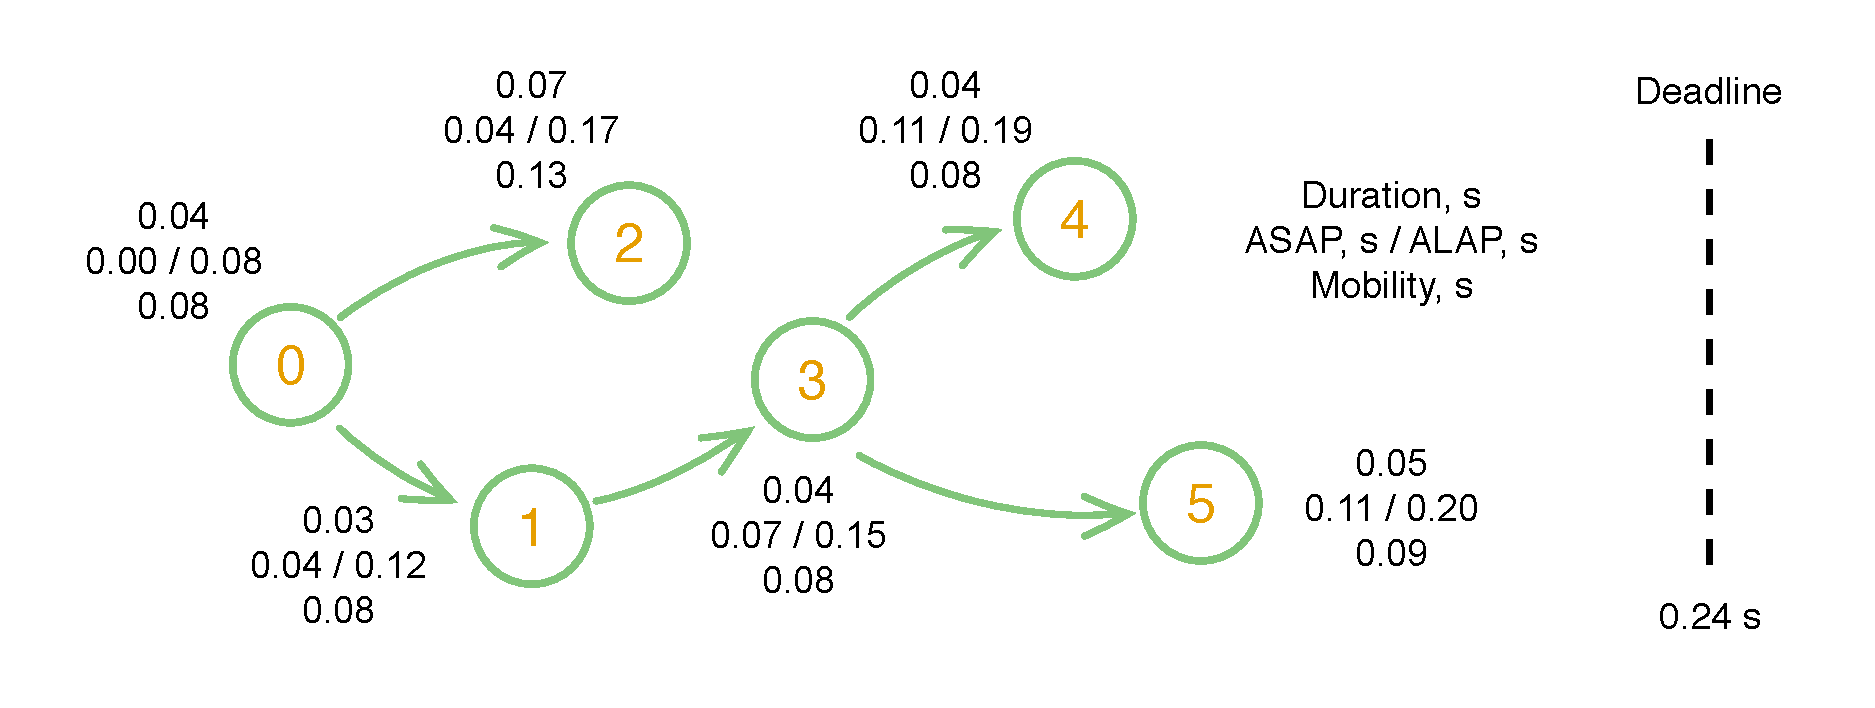
\includegraphics[width=0.8\linewidth]{assets/task-graph.pdf}
  }
  \vspace{-15pt}

  \subfloat[Alternative mappings and schedules.]{
    \label{fig:motivation}
    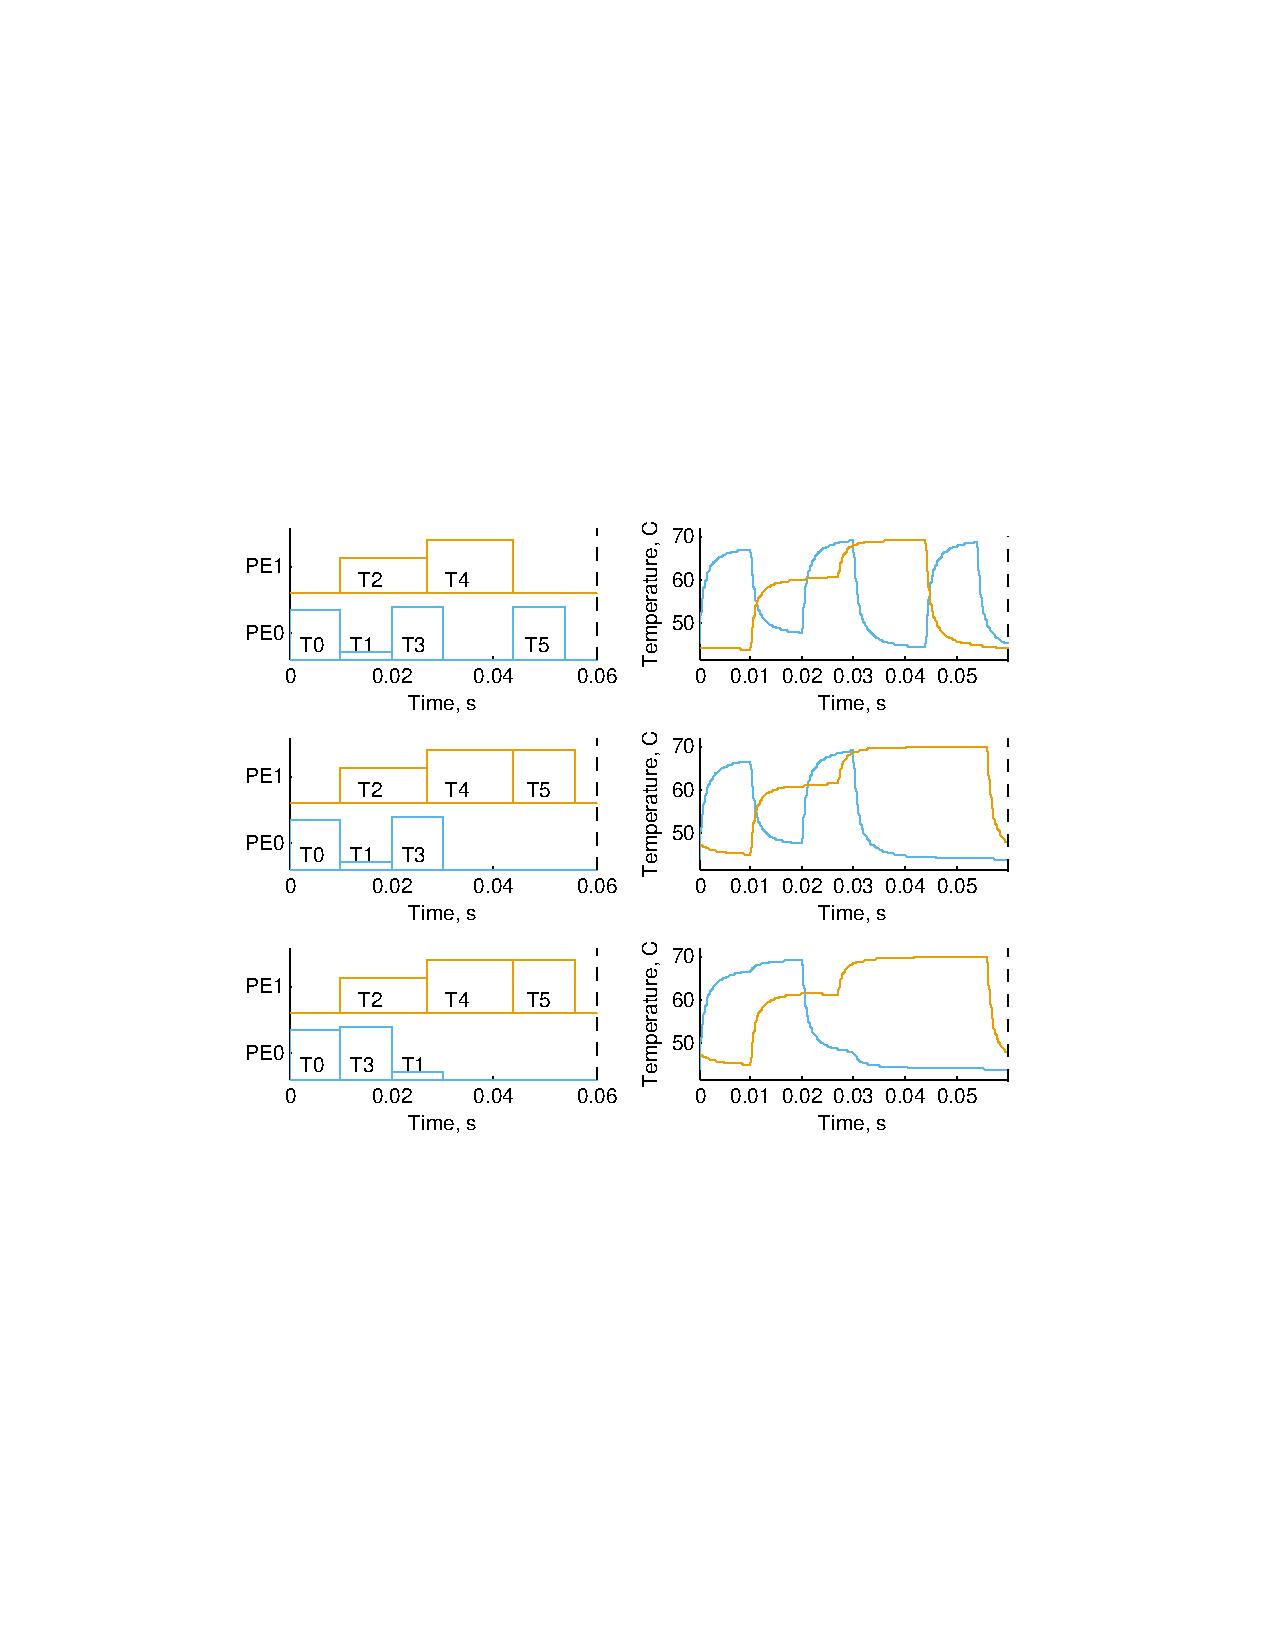
\includegraphics[width=0.8\linewidth]{assets/motivation.pdf}
  }
  \vspace{5pt}
  \caption{Motivational example.}
  \vspace{15pt}
\end{figure}


\subsection{Genetic Algorithm}
The optimization procedure is held by a genetic algorithm (GA) \cite{schmitz2004} that varies mapping and scheduling of the application in order to maximize the MTTF of the system. Each chromosome is a vector of $2 \times N_t$ elements, where the first half encodes priorities of the tasks and the second represents a mapping. The population contains $4 \times N_t$ individuals that are initialized partially randomly and partially based on the mobility of the tasks \cite{schmitz2004}. Each generation, a number of individuals, called parents, are chosen for breeding by the tournament selection with the number of competitors proportional to the population size. The parents undergo the 2-point crossover with $0.8$ probability and uniform mutation with $0.05$ probability. The evolution mechanism follows the elitism model where the best individual always survives. The stopping condition is an absence of improvement within $200$ successive generations.

A chromosome is evaluated in a number of steps. First, the decoded priorities and mapping are given to a list scheduler that produces schedules for each of the cores. If the schedules do not respect the deadline of the application, the solution is penalized proportionally to the delay and is not further evaluated; otherwise, based on the parameters of the architecture and tasks, a dynamic power profile is obtained. Having the dynamic power profile and taking into consideration the leakage power with the linear approximation from \secref{sec:leakage}, the corresponding SSDTP is computed by the CE method. Finally, the SSDTP is assessed in terms of the reliability model given in \equref{eq:mttf-system}, where the rainflow counting method is employed to count thermal cycles \cite{xiang2010}.


  \section{Experimental Results} \label{sec:results}
  \subsection{Computation Performance} \label{sec:results-ssdtp}
In this subsection we investigate the scalability properties of the proposed solution based on the CE method and compare it with one transient temperature simulation (TTS) of the application period, which is not sufficient to reach the SSDTP as it was shown in \secref{sec:hotspot-solution}. To perform the TTA, the HotSpot thermal simulator is used.

\image{scaling-time}{80 230 80 230}{Scalability with the application period for a quad-core architecture. The sampling interval is fixed to 1 millisecond where 1 second on the horizontal axis corresponds to 1000 steps in the power profile. The comparison is given on the semilogarithmic scale.}
\begin{itable}{scaling-time}{|r|r|r|r|r|}
  {Scalability with the application period shown in \figref{fig:scaling-time}.}
  {$\mathcal{T}$ --- the application period, CE --- the Condensed Equation method, TTS --- one Transient Temperature Simulation, NRMSE --- the Normalized Root Mean Square Error.}
  \hline
  $\mathcal{T}$, s & CE, ms & TTS, ms & Speedup, $\times$ & NRMSE, \% \\
  \hline
  \hline
  0.05 &  0.18 &   10.24 & 56.93 & 25.8 \\
   0.1 &  0.35 &   20.26 & 58.30 & 19.0 \\
   0.5 &  1.63 &   97.36 & 59.73 & 9.65 \\
     1 &  3.23 &  193.31 & 59.80 & 7.80 \\
     2 &  6.48 &  382.59 & 59.08 & 6.46 \\
     3 &  9.58 &  573.15 & 59.83 & 5.79 \\
     4 & 12.78 &  770.09 & 60.25 & 5.34 \\
     5 & 16.10 &  964.75 & 59.92 & 5.00 \\
     6 & 19.32 & 1146.87 & 59.36 & 4.72 \\
     7 & 22.51 & 1335.26 & 59.31 & 4.49 \\
     8 & 25.69 & 1536.91 & 59.82 & 4.28 \\
     9 & 28.94 & 1729.39 & 59.76 & 4.09 \\
    10 & 32.65 & 1921.14 & 58.83 & 3.93 \\
  \hline
\end{itable}
First, we vary the application period keeping the sampling interval constant and equal to 1 millisecond. The comparison for a quad-core architecture is given in \figref{fig:scaling-time} and \tabref{tab:scaling-time}. It can be seen that the CE method is roughly 60 times faster than one iteration of the TTA\footnote{All the experiments are done on a Linux machine with Intel\textregistered\ Core\texttrademark\ i7-2600 (3.4GHz, 4 cores, 8 threads) and 8Gb of RAM.}. The application period proportionally corresponds to the number of steps in the power profile (one second is equal to 1000 steps in the power profile in the above-mentioned example). Hence, we would see the same curves, if we were investigating the dependency on the power profile discretization.

\image{scaling-cores}{80 230 80 230}{Scalability with the number of cores. The application period is fixed to 1 second that corresponds to 1000 steps in the power profile. The comparison is given on the semilogarithmic scale.}
\begin{itable}{scaling-cores}{|r|r|r|r|r|}
  {Scalability with the number of cores shown in \figref{fig:scaling-cores}.}
  {$N_p$ --- the number of processing elements (cores), CE --- the Condensed Equation method, TTS --- one Transient Temperature Simulation, NRMSE --- the Normalized Root Mean Square Error.}
  \hline
  $N_p$ & CE, ms & TTS, ms & Speedup, $\times$ & NRMSE, \% \\
  \hline
  \hline
    1 &    0.99 &    97.00 & 97.93 &  25 \\
   10 &   16.46 &   632.50 & 38.44 &  41 \\
   20 &   46.00 &  1761.75 & 38.30 &  69 \\
   30 &   98.49 &  3472.21 & 35.25 & 102 \\
   40 &  172.69 &  5827.77 & 33.75 & 130 \\
   50 &  266.08 &  8771.93 & 32.97 & 142 \\
   60 &  380.95 & 12235.91 & 32.12 & 185 \\
   70 &  517.04 & 16363.54 & 31.65 & 220 \\
   80 &  675.21 & 21104.98 & 31.26 & 245 \\
   90 &  856.20 & 26415.77 & 30.85 & 277 \\
  100 & 1058.35 & 32329.09 & 30.55 & 308 \\
  \hline
\end{itable}
The second part of the comparison is the scalability with the number of processing elements shown in \figref{fig:scaling-cores} and \tabref{tab:scaling-cores}. It can be seen that the difference between computation times of the CE method and one TTS becomes smaller when the number of cores is increasing. At the same time the mismatch between the SSDTP and temperature profile produced by one TTA dramatically increases, which means that larger number of the TTA iterations is required to reach the same level of accuracy.

\subsection{Reliability Optimization}
The experimental setup is the following. Heterogeneous architectures and periodic applications are generated randomly \cite{dick1998} in such a way that the execution time of tasks is uniformly distributed between 1 and 50 milliseconds and the leakage power accounts for 30--55\% of the total power dissipation. The corresponding temperature variation lies between the ambient temperature of $27^{\circ}C$ and maximal temperature of $100^{\circ}C$.

In each of the experiments, we compare the optimized solution with the initial one that is obtained in the following way. First, we calculate the average execution time of each task among the processing elements. Then, we compute the mobility of the tasks and schedule the application according to it \cite{schmitz2004}. The mapping is done along with the scheduling where each task being considered is assigned to the earliest available core in the system. This combination of mapping and scheduling is the starting point for the future optimization. The deadline of the application is set according to the duration of the initial schedule with additional 5\%.

\begin{itable}{mttf-cores}{|r|r|r|r|r|}
  {Reliability optimization for different architectures}
  {$N_p$ --- the number of cores, $N_t$ --- the number of tasks, $t_{avg}$ --- the average computational time, $MTTF_{avg}$ --- the average MTTF improvement, $E_{avg}$ --- the average change in the energy consumption.}
  \hline
  $N_p$ & $N_t$ & $t_{avg}, m$ & $MTTF_{avg}$, \% & $E_{avg}$, \% \\
  \hline
   2 &   20 &   0.66 & 8123.29 & -13.50 \\
   4 &   40 &   2.04 & 7424.04 & -22.92 \\
   8 &   80 &  10.67 & 2819.45 & -21.88 \\
  16 &  160 &  25.38 &  915.11 & -13.78 \\
  32 &  320 &  89.59 &  442.49 &  -8.90 \\
  \hline
\end{itable}
In the first set of experiments, we change the number of cores while keeping the number of tasks per core constant and equal to 10. For each problem we have generated 20 random task graphs of a similar structure and found the average improvement of the MTTF. We also have measured the change in the consumed energy. The results are given in \tabref{tab:mttf-cores}. It can be observed that the temperature-unaware task allocation and scheduling dramatically decrease the lifetime of the device and the optimization based on the SSDTP is a must for an embedded system design framework. Although, the average improvement is decreasing with the growth of the complexity of the problem, it is still considerably high. Note that the energy efficiency of the system is not suffering from the optimization, on the contrary, we observed that the found solutions are generally better with comparison to the initial ones from this perspective.

\begin{itable}{mttf-tasks}{|r|r|r|r|r|}
  {Reliability optimization for different applications}
  {$N_p$ --- the number of cores, $N_t$ --- the number of tasks, $t_{avg}$ --- the average computational time, $MTTF_{avg}$ --- the average MTTF improvement, $E_{avg}$ --- the average change in the energy consumption.}
  \hline
  $N_p$ & $N_t$ & $t_{avg}, m$ & $MTTF_{avg}$, \% & $E_{avg}$, \% \\
  \hline
  4 &  20 & 0.93 & 13029.86 & -26.62 \\
  4 &  40 & 1.81 &  4311.02 & -22.15 \\
  4 &  80 & 0 & 0 & 0 \\
  4 & 160 & 0 & 0 & 0 \\
  4 & 320 & 0 & 0 & 0 \\
  \hline
\end{itable}
For the second set of experiments, we keep the quad-core architecture and vary the number of tasks within the application. The number of randomly generated task graphs per problem is 20. The average improvement of the MTTF along with the change in the energy consumption are given in \tabref{tab:mttf-tasks}. The observations to be made here are similar to the previous ones: taking into consideration the SSDTP of the system during the design stage can significantly prolong the MTTF without sacrificing the energy efficiency of the system.

\begin{itable}{mttf-comparison}{|r|r|r|r|r|}
  {Reliability optimization for different solution techniques}
  {$N_p$ --- the number of cores, $N_t$ --- the number of tasks, $MTTF^{CE}_{avg}$, $MTTF^{TTA}_{avg}$, and $MTTF^{SS}_{avg}$ --- the average improvements of the MTTF obtained by the CE method, TTA with HotSpot, and SS approximation, respectively.}
  \hline
  $N_p$ & $N_t$ & $MTTF^{CE}_{avg}$, \% & $MTTF^{TTA}_{avg}$, \% & $MTTF^{SS}_{avg}$, \% \\
  \hline
  4 &  20 & 0 & 0 & 0 \\
  4 &  40 & 0 & 0 & 0 \\
  4 &  80 & 0 & 0 & 0 \\
  4 & 160 & 0 & 0 & 0 \\
  4 & 320 & 0 & 0 & 0 \\
  \hline
\end{itable}
Finally, we compare the results of the optimization delivered by the CE method, TTA with HotSpot, and steady-state approximation (SS) discussed in \secref{sec:steady-state-approximation} for the same setup as in the previous set of experiments with the fixed architecture. The final solution found by the later two methods, TTA and SS, are reevaluated using the CE method and compared with the solutions found only by the CE approach. The results are summarized in \tabref{tab:mttf-comparison}. \todo{Obtain results and discuss.}


  \section{Conclusion} \label{sec:conclusion}
  The SSDTA is an essential part of the embedded system design. In this paper we formutated the problem and proposed an elegant anlytical technique to solve it. The solution is both accurate and fast enough to be a decent tool of the designer. Using the proposed approach, we conducted a temperature-aware reliability optimization based on the thermal cycling failure mechanism and shown that taking into consideration the temperature variations within a multicore platform can significantly prolong its lifetime without affecting its energy efficiency.


  \section{Acknowledgments}
  We would like to thank Prof. {\AA}ke Bj\"{o}rck from the Link\"{o}ping University in Sweden for the valuable discussions and suggestions about the analytical solution.

  \begin{thebibliography}{99}
  \bibitem{kreith2000}
    F. Kreith,
    ``CRC Handbook of Thermal Engineering,''
    \emph{CRC Press},
    2000.

  \bibitem{huang2006}
    W. Huang, S. Ghosh, S. Velusamy, K. Sankaranarayanan, K. Skadron, M. R. Stan,
    ``HotSpot: A Compact Thermal Modeling Methodology for Early-Stage VLSI Design,''
    \emph{IEEE Transactions on Very Large Scale Integration (VLSI) Systems},
    vol.~14, no.~5, pp.~501--513, May 2006.

  \bibitem{lu2004}
    Z. Lu, W. Huang, S. Ghosh, J. Lach, M. Stan, K. Skadron,
    ``Analysis of Temporal and Spatial Temperature Gradients for IC Reliability,''
    March 2004.

  \bibitem{srinivasan2004}
    J. Srinivasan , S. V. Adve , P. Bose , J. A. Rivers,
    ``The Impact of Technology Scaling on Lifetime Reliability,''
    \emph{International Conference on Dependable Systems and Networks},
    pp.~177--186, June 2004.

  \bibitem{liao2005}
    W. Liao, L. He, K. M. Lepak,
    ``Temperature and Supply Voltage Aware Performance and Power Modeling at Mictoarchitecture Level,''
    \emph{IEEE Transactions on Computer-Aided Design of Integrated Circuits and Systems},
    vol.~24, no.~7, pp.~1042--1053, July 2005.

  \bibitem{coskun2006}
    A. K. Coskun, T. S. Rosing, K. Mihic, G. De Micheli, Y. Leblebici,
    ``Analysis and Optimization of MPSoC Reliability,''
    \emph{Journal of Low Power Electronics},
    vol.~, no.~1, pp.~56--69, 2006.

  \bibitem{liu2007}
    Y. Liu, R. P. Dick, L. Shang, H. Yang,
    ``Accurate Temperature-Dependent Integrated Circuit Leakage Power Estimation is Easy,''
    \emph{DATE'07},
    2007.

  \bibitem{huang2009}
    L. Huang, F. Yuan, Q. Xu,
    ``Lifetime Reliablity-Aware Task Allocation and Scheduling for MPSoC Platforms,''
    \emph{DATE'09},
    June 2009.

  \bibitem{xiang2010}
    Y. Xiang, T. Chantem, R. P. Dick, X. S. Hu, L. Shang,
    ``System-Level Reliability Modeling for MPSoCs,''
    \emph{CODES+ISSS'10},
    October 2010.

  \bibitem{thiele2011}
    L. Thiele, L. Schor, H. Yang, I. Bacivarov,
    ``Thermal-Aware System Analysis and Software Synthesis for Embedded Multi-Processors,''
    \emph{DAC'11},
    June 2011.

  \bibitem{rao2007}
    R. Rao, S. Vrudhula,
    ``Performance Optimal Processor Throttling Under Thermal Constraints,''
    \emph{CASES'07}
    Septermer--October, 2008.

  \bibitem{hanumaiah2009}
    V. Hanumaiah, R. Rao, S. Vrudhala, K. S. Chatha,
    ``Throughput Optimal Task Allocation under Thermal Constraints for Multi-core Processors,''
    \emph{DAC'09},
    July 2009.

  \bibitem{bao2010}
    M. Bao, A. Andrei, P. Eles, Z. Peng,
    ``Temperature-Aware Idle Time Distribution for Energy Optimization with Dynamic Voltage Scaling,''
    \emph{DATE'10},
    March 2010.

  \bibitem{jedec2010}
    JEDEC Solid State Technology Association,
    ``Failure Mechanisms and Models for Semiconductor Devices,''
    \emph{JEDEC Publication},
    November 2010.

  \bibitem{hieu2004}
    N. Van Hieu,
    ``Multilevel Interconnect Reliability on the Effects of Electro-Thermomechanical Stress,''
    2004.

  \bibitem{press2007}
    W. H. Press, S. A. Teukolsky, W. T. Vetterling, B. P. Flannery,
    ``Numerical Recipes: The Art of Scientific Computing,''
    \emph{Cambridge University Press},
    third edition, 2007.

  \bibitem{umfpack2004}
    T. A. Davis,
    ``Algorithm 832: UMFPACK, an unsymmetric-pattern multifrontal method,''
    \emph{ACM Transactions on Mathematical Software},
    vol.~30, no.~2, pp.~196--199, June 2004.

  \bibitem{mazancourt1983}
    T. De Mazancourt, D. Gerlic,
    ``The Inverse of a Block-Circulant Matrix,''
    \emph{IEEE Transactions on Antennas and Propagation},
    vol.~AP–31, no.~5, pp.~808–810, September 1983.

  \bibitem{vescovo1997}
    R. Vescovo,
    ``Inversion of Block-Circulant Matrices and Circular Array Approach,''
    \emph{IEEE Transactions on Antennas and Propagation},
    vol.~45, no.~10, pp.~1565-–1567, October 1997.

  \bibitem{stoer2002}
    J. Stoer, R. Bulirsch,
    ``Introduction to Numerical Analysis,''
    \emph{Springer-Verlag, New York},
    third edition, 2002.

  \bibitem{schmitz2004}
    M. T. Schmitz, B. M. Al-Hashimi, P. Eles,
    ``System-Level Design Techniques for Energy-Efficient Embedded Systems,''
    \emph{Kluwer Academic Publishers},
    2004.

  \bibitem{chang2006}
    S.-C. Chang, S.-Y. Deng, J. Y.-M. Lee,
    ``Electrical Characteristics and Reliability Properties of Metal-Oxide- Semiconductor Field-Effect Transistors with Dy2O3 Gate Dielectric,''
    \emph{Apply Physics Letters},
    no.~85, August 2006.

  \bibitem{ciappa2003}
    M. Ciappa, F. Carbognani, W. Fichtner,
    ``Lifetime Prediction and Design of Reliability Tests for High-Power Devices in Automotive Applications,''
    \emph{IEEE Transactions on Device and Materials Reliability},
    vol.~3, no.~4, pp.~191--196, December 2003.

  \bibitem{dick1998}
    R. P. Dick, D. L. Rhodes, W. Wolf,
    ``TGFF: Task Graphs for Free,''
    \emph{CODES/CASHE'98},
    March 1998.
\end{thebibliography}

\end{document}
